%% packages
\documentclass{article}
\usepackage[a4paper, left=2.0cm, right=2.0cm, top=3.5cm]{geometry}
\usepackage[ngerman]{babel}
\usepackage{graphicx}
\usepackage{multicol}
\usepackage{amssymb}
\usepackage{titlesec}
\usepackage{wrapfig}
\usepackage{blindtext}
\usepackage{lipsum}
\usepackage{caption}
\usepackage{listings}
\usepackage{fancyhdr}
\usepackage{nopageno}
\usepackage{authblk}
\usepackage{amsmath} % tons of math stuff
\usepackage{mathtools} % e.g. alignment within matrix
%\usepackage{bm} % provides shorthand for bold in math mode
\usepackage{dsfont} % \mathds makes double stroke digits
\usepackage{esdiff} % provides \diff
%\usepackage[ISO]{diffcoeff}
\usepackage{xcolor}
\usepackage{csquotes} % e.g. provides \enquote
\usepackage[separate-uncertainty=true]{siunitx} % units
\usepackage{xcolor} % colored text
\usepackage{csvsimple}
\usepackage{subcaption}
\usepackage{physics}
\usepackage{hyperref}
\usepackage{nameref}
\hypersetup{colorlinks=true, linkcolor=black, pdfhighlight={/N}}
\usepackage{tcolorbox}
\usepackage{amsthm}
\usepackage{float}
\usepackage{enumitem}
\usepackage{booktabs}

% \sisetup{
%   scientific-notation = auto,  % Automatically use scientific notation for large/small numbers
%   output-exponent-marker = \text{e}  % (optional) for formatting the exponent symbol
% }

%\fancyhf[]{}

%% custom stuff
% own units
\DeclareSIUnit \VSS {\ensuremath{V_\mathrm{SS}}}
\DeclareSIUnit \VS {\ensuremath{V_\mathrm{S}}}
\DeclareSIUnit \Veff {\ensuremath{V_\mathrm{eff}}}
\DeclareSIUnit \Vpp {\ensuremath{V_\mathrm{pp}}}
\DeclareSIUnit \Vp {\ensuremath{V_\mathrm{p}}}
\DeclareSIUnit \VRMS {\ensuremath{V_\mathrm{RMS}}}
\DeclareSIUnit \ASS {\ensuremath{A_\mathrm{SS}}}
\DeclareSIUnit \AS {\ensuremath{A_\mathrm{S}}}
\DeclareSIUnit \Aeff {\ensuremath{A_\mathrm{eff}}}
\DeclareSIUnit \App {\ensuremath{A_\mathrm{pp}}}
\DeclareSIUnit \Ap {\ensuremath{A_\mathrm{p}}}
\DeclareSIUnit \ARMS {\ensuremath{A_\mathrm{RMS}}}

% change subsection numbering to capital letters
\newcommand{\subsectionAlph}{ \renewcommand{\thesubsection}{\arabic{section}.\Alph{subsection}} }
% change subsection numbering to lowercase letters
\newcommand{\subsectionalph}{ \renewcommand{\thesubsection}{\arabic{section}.\alph{subsection}} }
% change subsubsection numbering to lowercase letters
\newcommand{\subsubsectionalph}{ \renewcommand{\thesubsubsection}{\arabic{section}.\arabic{subsection}.\alph{subsubsection}} }
% own fig. that works with multicols
\newenvironment{Figure}
  {\par\medskip\noindent\minipage{\linewidth}}
  {\endminipage\par\medskip}
\newcommand*{\inputPath}{./plot} % prepend this command to the argument of all input commands
\graphicspath{ {./images/}{./figure/}{../plot/}{../../plot/}{../../latex/assets/}{./assets/} }
% own enviroment for definitions
\newenvironment{definition}[1]
{\begin{quote} \noindent \textbf{\textit{#1\ifx&#1& \else : \fi}} \itshape}
{\end{quote}}



% own commands
% \newcommand{\rarr}{$\to\,$} %A$\,\to\,$B
\newcommand{\defc}{black}
\newcommand{\colorT}[2][blue]{\color{#1}{#2}\color{\defc}}
\newcommand{\redq}{\color{red}(?)\color{\defc}}
\newcommand{\question}[1]{\colorT[purple]{\textbf{(#1)}}}
\newcommand{\todo}[1]{\colorT[red]{\textbf{(#1)}}}
\newcommand{\mr}{\mathrm}


%% preparation


%dachte wir können hier durchführung und gleich Auswertung der einzelnen Versuchsaufgaben schreiben und im Fazit ein gesamtfazit

%\displaystyle \lim_{x \to \infty}

\begin{document}
    \title{Elektronikpraktikum \\ \textbf{Versuch 1: Ausbreitung von Signalen auf Leitungen}}
    \author[1]{Carlos Pascua \thanks{s87cpasc@uni-bonn.de}}
    \author[1]{Anna Maróti\thanks{s32amaro@uni-bonn.de}}
    \author[1]{Cornelius Heiming\thanks{s64cheim@uni-bonn.de}}
    \affil[1]{Uni Bonn}
    %\date{\today}
	\pagenumbering{gobble}
    \begin{titlepage}
     \maketitle   
    \end{titlepage}
        
\tableofcontents
\newpage
\pagenumbering{arabic}

\pagestyle{fancy}
\fancyhead[R]{\thepage}
\fancyhead[L]{\leftmark}

\section{Theorie}

\subsection*{Einführung}

In diesem Versuch wird die Ausbreitung von Signalen in verschiedenen Kabeln, wie beispielsweise in Koaxialkabeln, 
untersucht. Des Weiteren werden Wechselspannungssignale bei verschiedenen Widerständen und unterschiedlichen 
Leitungsenden analysiert, um ihr Verhalten zu verstehen.

%Jegliche Schaltkreise, sowie das Diagramm \ref{Dämpfung Kabelsorten Diagramm} entstammen aus \cite{skript:ElektronikPraktikum}.
% das hatten noah und ich das letzte mal geschrieben um das skript zu zitieren. aber hier haben wir eine andere Zitierform


\subsection*{Koaxialleiter}

Ein Koaxialleiter setzt sich aus einem inneren und einem äußeren zylindrischen Leiter zusammen. Sie sind konzentrisch angeordnet und werden von einem Dielektrikum voneinander getrennt. Das Dielektrikum isoliert die Leiter voneinander, welches die Signalübertragung unterstützt, da es die elektrische Feldstärke zwischen den Leitern minimiert wird. 
Die Kapazität und Induktivität von einem Koaxialleiter entspricht:

    \begin{equation}
        C= \epsilon_r \epsilon_0 l \frac{2\pi}{\ln{\frac{R_a}{R_i}}}
    \end{equation}
    
    \begin{equation}
        L= \mu_r \mu_0  \frac{\ln{R_a/R_i}}{2\pi}
    \end{equation}
    
wobei $l$ Länge des Kabels, $R_{a/i}$ Radien der Leitern,$\epsilon_0 = 8,85\cdot10^{-12} \frac{As}{Vm}$ die elektrische Feldkonstante und $\mu_0 = 4\pi\cdot 10^{-7} \frac{Vs}{Am}$ die magnetischen Feldkonstante ist.

Den Kabel kann man auch als mehreren zusammenhängenden LC-Gliedern approximieren. Die Länge hat einen proportionalen Einfluss auf die Impedanz und Admittanz des Kabels. Eine Weitere wichtige Größe ist der Verlustleitwert (Ableitung) $G$. Dieser ist der ohmsche Leitwert zwischen dem Hin- und Rückleiter. \\
Des Weiteren gibt wird der Kabel noch über seine Übertragungsfähigkeit bestimmt, welches durch den Wellenwiderstand Z, der Verzögerungszeit und der Dämpfung definiert ist. Für den Wellenwiderstand gilt mit der Induktivität $L^{\prime}$ und Kapazität $C^{\prime}$ pro Längeneinheit:
\[ Z = \sqrt{\frac{L^{\prime}}{C^{\prime}}}= \sqrt{\frac{\mu_r \mu_0}{\epsilon_r \epsilon_0}}\cdot \frac{\ln{R_a/R_i}}{2\pi}\]
Die Verzögerungszeit ist definiert als die Zeitdifferenz der einlaufenden und reflektierten Welle zusammen. 
Die rücklaufende Welle kann mit der Dämpfungskonstante $ \alpha$ gedämpft werden:
\begin{equation*}
    \Upsilon = \alpha + i \beta
\end{equation*}


\subsection*{Wellenausbreitung und Leitungsabschluss}
Anhand des Superpositionprinzips können Strom und Spannung durch eine Überlagerung einer hin- und \\ rücklaufenden Welle beschrieben werden.
\begin{equation*}
   U(x,t) = U_h(x,t) + U_r(x,t)= (U_{h0} e ^{-\Upsilon x} + U_{r0} e ^{-\Upsilon x}) e^{i \omega t} 
\end{equation*}
sowie
\begin{equation*}
    I(x,t) = (U_{h0} e^{-\Upsilon x} + U_{r0} e^{-\Upsilon x}) \cdot \sqrt{\frac{G^{\prime}+ i \omega C^{\prime}}{R^{\prime}+ i \omega L^{\prime}}}e^{i \omega t}= I_h(x,t) + I_r(x,t)
\end{equation*}
Wegen dieser Überlagerung sind der Leitungsabschluss und dessen Reflektionsgrad  sehr bedeutsam in der Elektrotechnik.

\subsection*{Angepasster Anschluss}
$R_A = Z$\\
Der Abschlusswiderstand $R_A$ entspricht dem Wellenwiderstand $Z$ des Kabels. Hierdurch überträgt sich die gesamte Energie des Kabels an den Verbraucher und die Welle wird nicht reflektiert, da der Verbraucher wie eine Weiterführung des Kabels entspricht und die Welle weiter den Kabel durchdringt.


\subsection*{Offene Leitung}
$R_A = \infty$\\
Es wird kein Strom an den Verbraucher übertragen, da der Abschlusswiderstand Unendlich entspricht. Hierdurch wird die gesamte Energie der Welle in gleicher Phase zurückreflektiert. Die rücklaufende Welle ist genau so groß wie die hinlaufende Welle.



\subsection*{Kurzschluss }
$R_A= 0 \Omega$\\
Bei einem Kurzschluss entspricht der der Abschlusswiderstand $ 0 \Omega$. Hierdurch wird die rücklaufende Welle phasenverschoben reflektiert. Sie entspricht der Inversen der hinlaufenden Welle, weshalb es zu einer destruktiven Überlagerung kommt.

\section{Voraufgaben}

\subsection*{Aufgabe A}
\begin{equation}
    v_{ph}= \frac{1}{\sqrt{L^{\prime}C^{\prime}}}= \frac{1}{\epsilon_0\mu_0}\cdot \frac{1}{\epsilon_r\mu_r} =c_0 \cdot \frac{1}{\epsilon_r\mu_r}
\end{equation}
Um möglichst große Verzögerungszeiten zu bekommen, muss die Phasengeschwindigkeit verkleinert werden und die Leitungslänge l vergrößert werden. Des Weiteren ist $t \propto L^{\prime}\propto C^{\prime}$. Außerdem kann man ableiten, dass man für eine große Verzögerungszeit das Kabel ein hohes Dielektrikum haben sollte, da dieses die Dielektrizität und Permeabilität erhöht wozu t auch proportional ist. 


\subsection*{Aufgabe B}
Für den Wellenwiderstand gilt: 
\begin{equation}
    Z = \sqrt{\frac{L^{\prime}}{C^{\prime}}} = \frac{\mu_0 \mu_r}{\epsilon_0\epsilon_r}\cdot \frac{\ln{\frac{R_a}{R_i}}}{2\pi}
\end{equation}

Somit löst die Veränderung der Verzögerungszeit durch die Parameter aus Aufgabe A, eine Veränderung für den Wellenwiderstand aus.Wenn die Induktivität oder Permeattivität erhöht wird, dann erhöht sich der Wellenwiderstand. Falls die Kapazität oder die Dielektrizität erhöht werden, verkleinert sich der Wellenwiderstand. Die Leitungslänge l hat keinen Einfluss auf den Widerstand.



\subsection*{Aufgabe C}
Der Eingangswiderstand ist unabhängig vom Kabel. Also wenn der Kabel abgeschlossen ist $R_A = Z$, dann $R_A = Z= R_{in}$


\subsection*{Aufgabe D}


Im Idealfall gelten folgende Eigenschaften für einen Leiter:
\\ $\frac{\mathrm{R_A}}{\mathrm{R_1}} = 2,3$, $\epsilon_0 = 1,5$, $\mu_0 = 1,5$. 
\\
Für die Phasengeschwindigkeit $v_{ph}$ gilt: 
\begin{equation*}
    v_{ph} = \frac{1}{\sqrt{L'\cdot C'}} = \frac{1}{\sqrt{\epsilon_r \epsilon_0 \mu_r \mu_0}} = c_o \cdot \frac{1}{\sqrt{\epsilon_r \mu_r}} = 2 \cdot 10^8  \frac{m}{s} 
\end{equation*}
Für den Wellenwiderstand gilt:
\begin{equation}
    Z = \sqrt{{\frac{L'}{C'}}} = Z_{frei} \cdot \frac{\ln(\frac{R_A}{R_1})}{2\pi} \approx 49,98\Omega
\end{equation}

Also ist die Verzögerungszeit pro Meter: $t_v = 5 \cdot 10^{-9} \frac{s}{m}$

\section{Versuchsaufbau, -durchführung, Messwerte und Auswertung}
		
		
% === Aufgabe 1 ===
		\subsection{Versuchsaufgabe 1: Differenzierglied}


			\begin{figure}[H]
				\centering
				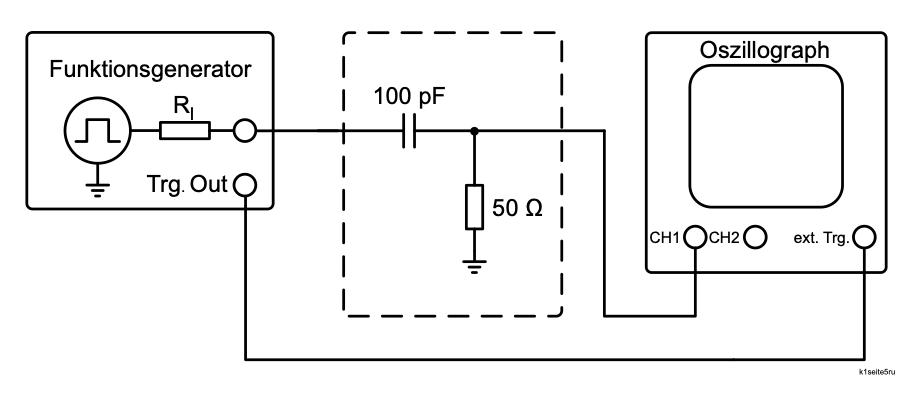
\includegraphics[width=0.5\textwidth]{figs/Aufbau_1_1_Differenzierglied.png}
				\caption{Schaltplan eines Differenzierglieds~\cite{anleitung}}
				\label{fig:aufbau_1_1_differenzierglied}
			\end{figure}
			Ein RC-Glied wird (ohne $\SI{2.2}{\kilo\ohm}$ Abschluss) zwischen einen Funktionsgenerator und einen Oszillographen geschaltet. Der Funktionsgenerator wird auf eine Frequenz von $\SI{200}{\kilo\hertz}$ eingestellt. Dann wird das Oszillogramm gezeichnet und dasselbe mit dem $\SI{2.2}{\kilo\ohm}$ Abschlusswiderstand wiederholt.
			
			
			\begin{figure}[H]
				\centering
				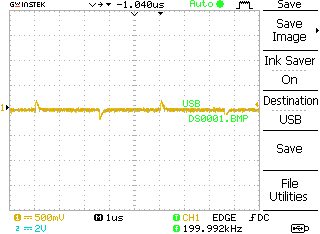
\includegraphics[width=0.5\textwidth]{MesswerteVersuch1/DS0001.png}
				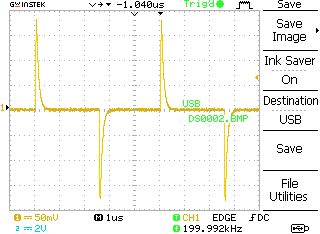
\includegraphics[width=0.5\textwidth]{MesswerteVersuch1/DS0002.png}
				\caption{Differenzierglied mit Abschlusswiderstand (unten vergrößerte Ordinate)}
				\label{fig:DS0001,2}
			\end{figure}
			\begin{figure}[H]
				\centering
				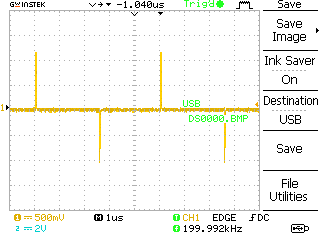
\includegraphics[width=0.8\textwidth]{MesswerteVersuch1/DS0000.png}
				\caption{Differenzierglied ohne Abschlusswiderstand}
				\label{fig:DS0000}
			\end{figure}
			
            Wie in Abbildung \ref{fig:DS0000} zu erkennen ist, wird das Rechtecksignal des Funktionsgenerators durch das Differenzierglied in ein Impulsignal umgewandelt. Die Spikes sind hierbei gut zu erkennen. Das Rechtecksignal, was vom Signalgenerator ausgesandt wird, besteht aus Sinusfuktionen mit verschiedenen Frequenzen. Das RC-Glied, welches als Hochpass agiert, filtert nun die niedrige Frequenzen aus, woraus die Plateaus bestanden, aus. Aus diesem Grund wird das Signal differenziert und es bleiben nur noch die Peaks, die aus hohen Frequenzen bestehen übrig.
            Im Fall des Abschlusswiderstands, sind die Impulse schwächer(vgl. Abb. \ref{fig:DS0001,2} oben) und deren Abfall ist flacher (vgl. Abb.\ref{fig:DS0001,2} unten).
            Dies ist darauf zurückzuführen, dass der Abschlusswiderstand den Stromfluss behindert und weil sich der Kondensator langsamer entlädt. Der Abschlusswiderstand hat also eine dämpfende Wirkung auf das Signal.
			%TODO: Messwerte & Auswertung
	
\clearpage
% === Aufgabe 2 ===

\subsection{Versuchsaufgabe 2: Impulse auf Kabeln} 

			
			\begin{figure}[H]
				\centering
				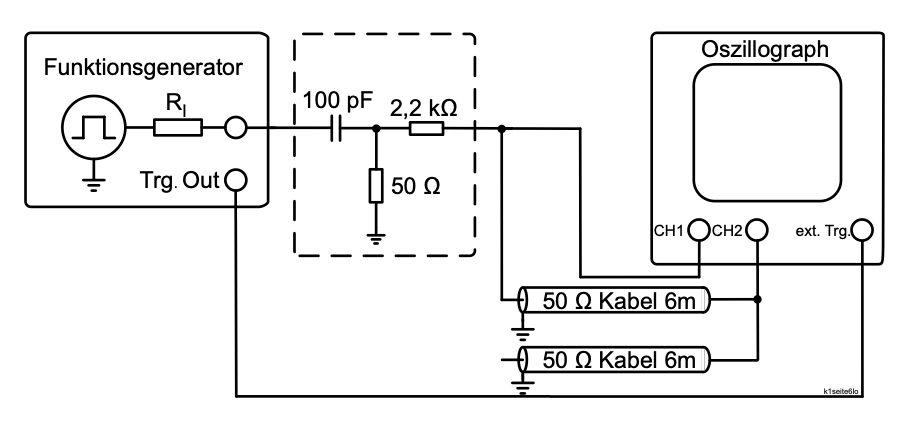
\includegraphics[width=0.8\textwidth]{figs/Aufbau_1_2_Impulse_auf_Kabeln.png}
				\caption{Schaltplan für ein Kabel mit zwei offenen Enden~\cite{anleitung}}
				\label{fig:aufbau_1_1_impulseAufKabeln}
			\end{figure}
			Jetzt sollen die Impulse auf einem an beiden Enden offenen Kabel untersucht werden. Dazu wird ein Funktionsgenerator, welcher im Rechteckmodus mit $\SI{100}{\kilo\hertz}$ betrieben wird, vor ein RC-Glied mit Abschluss, welches als Impulsgeber dient, geschaltet. Diese Impulse werden einerseits im CH1 des Oszillographen angezeigt, andererseits durch zwei hintereinandergeschaltete Kabel mit jeweils $\SI{50}{\ohm}$ Wellenwiderstand geschickt. Zwischen den beiden Kabeln wird der Oszillograph im CH2 geschaltet. Der Funktionsgenerator dient als externer Trigger für den Oszillographen, die beiden Kanäle werden mit derselben Empfindlichkeit betrieben.
			
			Auf der größeren Zeitachse (vgl. Abb. \ref{fig:DS0004}) kann man die Impulse des Funktionsgenerators wiedererkennen. Hier klingen diese nicht instantan durch die Darstellung im Oszillographen ab, sondern wandern durch die beiden Kabel, sodass nur ein Teil der Amplitude im Oszillographen ankommt. In der detaillierteren Darstellung (vgl. Abb. \ref{fig:DS0005}) kann man nun die einzelnen Durchläufe durch die beiden Kabel erkennen. Besonders gut dabei zu sehen ist, dass der Impuls den Punkt zwischen den beiden Kabeln doppelt so häufig passiert, wie den Punkt am Anfang des Kabels. Das macht also eine tatsächliche Bewegung des Signales über die Länge der Kabel deutlich. Dies kann man auch aus der Verzögerung der beiden Signale relativ zueinander erkennen, die in etwa der Hälfte der Periode vom Mittelpunkt bzw. einem Viertel der Periode vom Anfang des Kabels entspricht. 
			
			\begin{figure}[H]
				\centering
				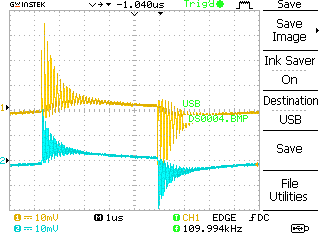
\includegraphics[width=0.8\textwidth]{MesswerteVersuch1/DS0004.png}
				\caption{Impulse auf Kabeln (Übersicht ($\SI{1}{\micro\second\per\centi\meter}$))}
				\label{fig:DS0004}
			\end{figure}
			\begin{figure}[H]
				\centering
				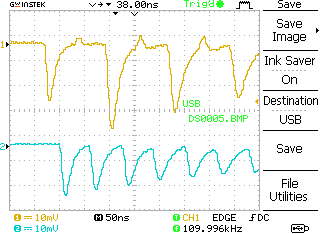
\includegraphics[width=0.8\textwidth]{MesswerteVersuch1/DS0005.png}
				\caption{Impulse auf Kabeln (Detailansicht ($\SI{0.05}{\micro\second\per\centi\meter}$))}
				\label{fig:DS0005}
			\end{figure}
		
\clearpage
% === Aufgabe 3 ===

\subsection{Versuchsaufgabe 3: Leitungsabschluss, Verzögerungszeit}
			
			\begin{figure}[H]
				\centering
				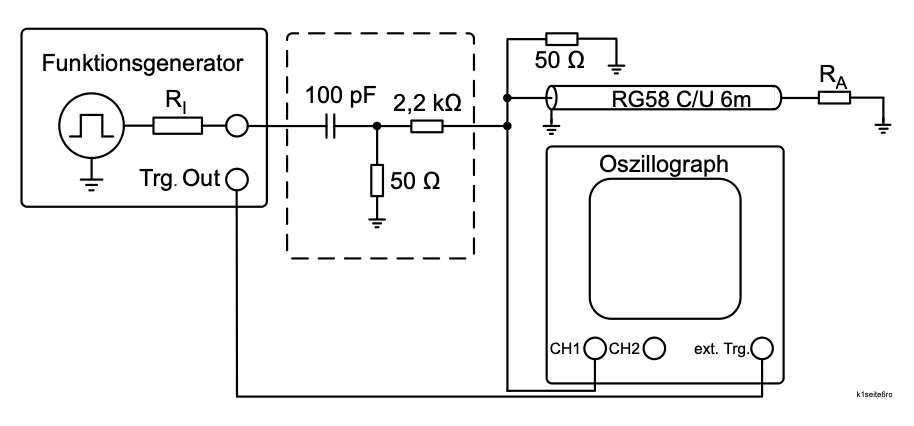
\includegraphics[width=0.8\textwidth]{figs/Aufbau_1_3_Leitungsabschluss.png}
				\caption{Schaltplan für ein Kabel mit einem offenen und einem geschlossenen Ende~\cite{anleitung}}
				\label{fig:aufbau_1_3_leitungsabschluss}
			\end{figure}
			Nun wird die Auswirkung unterschiedlicher Leitungsabschlüsse auf die Impulse untersucht. 
            Dazu wird weiterhin extern getriggert, der Impulsgenerator wird auch an CH1 angeschlossen. 
            Statt der beiden Kabel wird jetzt mittels eines T-Stücks ein Verzögerungskabel mit $\SI{50}{\ohm}$ 
            Wellenwiderstand und $\SI{6}{\meter}$ Länge verwendet, welches am anderen Ende mit einem Widerstand 
            $R_\mathrm{A} = \SI{50}{\ohm}$ abgeschlossen ist. Es für jede der folgenden Anordnungen mit und 
            ohne einem zusätzlichen Widerstand von $\SI{50}{\ohm}$ parallel zum Kabel gemessen:
			\begin{enumerate}[label=\alph*]
				\item Offenes Ende
				\item Offenes Ende im Detail ($\times 10$)
				\item Kurzgeschlossenes Ende
				\item Kurzgeschlossenes Ende \& variierende Frequenzen (Zeitablenktung von $\SI{0.2}{\micro\second\per\centi\meter}$)
			\end{enumerate}

            Ist beim Aufbau kein Anpassungswiderstand vorhanden, wird das Signal in gleicher Phase reflektiert. Schließt man aber den Anpassungswiderstand ein, werden keine Reflexionen mehr sichtbar sein, sondern zwei getrennte Pulse.
Mit Abbildung (/ref) lassen sich die gedämpften Peaks erkennen. Es ist ersichtlich, dass die Schwingungen deutlich schneller abklingen als ohne Anpassungswiderstand, was zu erwarten ist, da der Widerstand als Verbraucher wirkt und das Signal weiter dämpft.
\\ Zudem ist zu erkennen, dass die Amplitude mit der Zeit abnimmt, was auf die Dämpfung der Leitung zurückgeführt werden kann.
				%TODO: Auswertung 3(a)
				\begin{figure}[H]
					\centering
					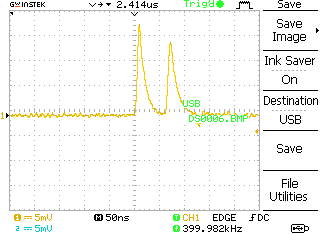
\includegraphics[width=0.5\textwidth]{MesswerteVersuch1/DS0006.png}
					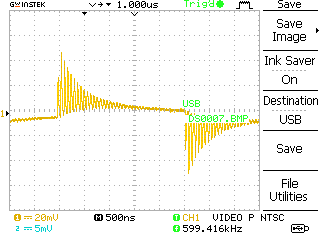
\includegraphics[width=0.5\textwidth]{MesswerteVersuch1/DS0007.png}
					\caption{Leitungsabschluss offenes Ende (oben: mit Anpassunsgwiderstand, unten: ohne Anpassungswiderstand)}
					\label{fig:DS0006,7}
				\end{figure}


               
                \clearpage
                Zunächst ist eine genauere Untersuchung der Impulsen gewollt. Dies wird ermöglicht, indem eine schnellere Zeitablenkung 
                des Oszillographen gewählt wird ($x10$ hereingezoomt). \\
                Nun kann man in der Abbildung \ref*{fig:DS0009.8} die 
                einzelnen Impulsen jeweils unterscheiden. Mit Anpassungswiderstand sieht man wieder genau 2 Impulse, die die 
                reflektierte und echte Siganle beschreiben. Es ist hier auch ersichtlich, dass die Zeit zwischen Amplituden, 
                bwz der Abstände dazwischen konstant bleibt. 
				%TODO: Auswertung 3(b)
				\begin{figure}[H]
					\centering
					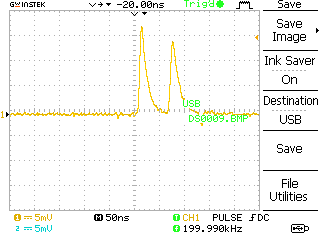
\includegraphics[width=0.5\textwidth]{MesswerteVersuch1/DS0009.png}
					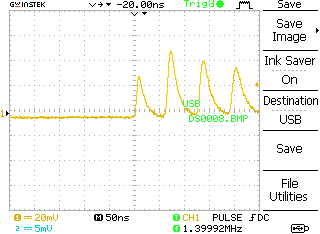
\includegraphics[width=0.5\textwidth]{MesswerteVersuch1/DS0008.png}
					\caption{Leitungsabschluss offenes Ende (oben: mit Anpassunsgwiderstand, unten: ohne Anpassungswiderstand) vergrößert}
					\label{fig:DS0009.8}
				\end{figure}

                \clearpage 

        Nun wird der ganze Vorgang wiederholt, mit der kleinen Änderung, dass das 
                Kabel am Ende mit einem Kurzchlussstrecker angeschlossen wird. Dies erfolgt 
                die folgenden Bilder:  
                
				%TODO: Auswertung 3(c)
				\begin{figure}[H]
					\centering
					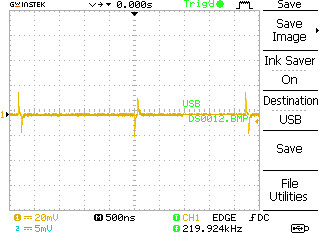
\includegraphics[width=0.5\textwidth]{MesswerteVersuch1/DS0012.png}
					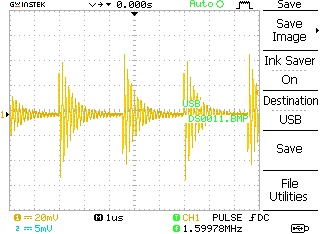
\includegraphics[width=0.5\textwidth]{MesswerteVersuch1/DS0011.png}
					\caption{Leitungsabschluss kurzgeschlossenes Ende (oben: mit Anpassunsgwiderstand, unten: ohne Anpassungswiderstand)}
					\label{fig:DS000}
				\end{figure}
                In den Abbildungen \ref*{fig:DS0006,7} und \ref*{fig:DS000} lässt sich der Unterschied zwischen offenem und 
                kurzgeschlossenem Leitungsende sehr gut erkennen. Bei offenem Ende ohne 
                Anpassungswiderstand (Abbildung \ref*{fig:DS0006,7} unten) treten deutliche gleichphasige 
                Reflexionen auf. Wird hingegen ein Anpassungswiderstand verwendet 
                (Abbildung \ref*{fig:DS0006,7} oben), wird die Reflexion stark gedämpft. Es bleibt nur 
                ein einzelner, gedämpfter Impuls sichtbar. Im Gegensatz dazu zeigt das 
                kurzgeschlossene Ende ohne Anpassung (Abbildung \ref*{fig:DS000} unten) eine gegenphasige 
                Reflexion auf, welches an den negativen Signalpeaks zu erkennen ist. Auch 
                hier führt der Anpassungswiderstand (Abbildung \ref*{fig:DS000} oben) zu einer starken 
                Dämpfung und einem sauberen Signalverlauf. Diese Unterschiede lassen sich 
                durch die Kabelanschlüsse erklären.
\clearpage
                Zuletzt variiert man die Frequenz ein wenig und beobachtet das 
                Oszillogrammgraphen bei einer festen Zeitablenkung von ungefähr $0,2 \mu s/cm$. 
                In unseren Fall haben wir uns für $250ns$ entschieden. Bei solcher Einstellung 
                bekommt man die folgenden Bilder: 
				\begin{figure}[H]
					\centering
					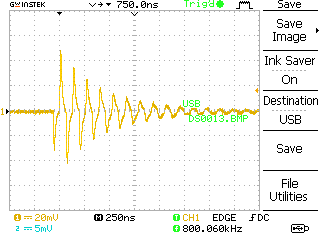
\includegraphics[width=0.5\textwidth]{MesswerteVersuch1/DS0013.png}	

					\caption{Leitungsabschluss kurzgeschlossenes Ende, Frequenz: $\SI{100}{\kilo\hertz}$}
					\label{fig:DS0013}
				\end{figure}
				\begin{figure}[H]
					\centering
					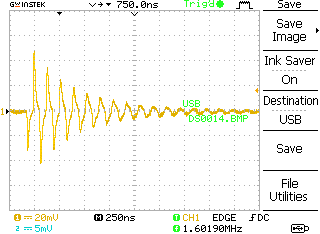
\includegraphics[width=0.5\textwidth]{MesswerteVersuch1/DS0014.png}	

					\caption{Leitungsabschluss kurzgeschlossenes Ende, Frequenz: $\SI{200}{\kilo\hertz}$}
					\label{fig:DS0014}
				\end{figure}

                Für die Verzögerungszeit gilt: 
                \[
t_{V,\text{erz}} = \frac{\Delta t}{2 \cdot l} = \frac{70\,\text{ns}}{2 \cdot 6\,\text{m}} = \frac{70\,\text{ns}}{12\,\text{m}} \approx 5{,}83\,\frac{\text{ns}}{\text{m}}
\]
Für die Fehlerrechnung wird die Gausschen Fehlerfortpflanzung angewendet, für $\Delta(\Delta t)=10ns$ und $\Delta l=0.1m$
\\ Dies erfolgt:

\[
\Delta t_{V,\text{erz}} =
\sqrt{
\left( \frac{\partial t_V}{\partial \Delta t} \cdot \Delta(\Delta t) \right)^2 +
\left( \frac{\partial t_V}{\partial l} \cdot \Delta l \right)^2
}
=
\sqrt{
\left( \frac{1}{2l} \cdot \Delta(\Delta t) \right)^2 +
\left( \frac{\Delta t}{2l^2} \cdot \Delta l \right)^2
}
\]

\[
=
\sqrt{
\left( \frac{1}{2 \cdot 6\,\text{m}} \cdot 10\,\text{ns} \right)^2 +
\left( \frac{70\,\text{ns}}{2 \cdot 6^2\,\text{m}^2} \cdot 0{,}1\,\text{m} \right)^2
}
\approx \sqrt{0{,}7034} \approx 0{,}84\,\frac{\text{ns}}{\text{m}}
\]
Alles zusammen:\\
\[
t_{V,\text{erz}} = (5{,}83 \pm 0{,}84)\,\frac{\text{ns}}{\text{m}}
\]
Unser experimenteller Wert passt gut mit dem Literaturwert aus der Anleitung \cite{anleitung} 
von ${V_\text{theo}} = 5\,\frac{\text{ns}}{\text{m}}$, da der Literaturwert in der Unsicherheit unseren errechneten Wertes liegt. 


				\begin{figure}[H]
					\centering
					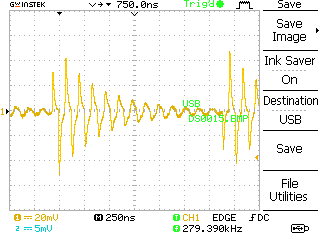
\includegraphics[width=0.5\textwidth]{MesswerteVersuch1/DS0015.png}	

					\caption{Leitungsabschluss kurzgeschlossenes Ende, Frequenz: $\SI{300}{\kilo\hertz}$}
					\label{fig:DS0015}
				\end{figure}
				\begin{figure}[H]
					\centering
					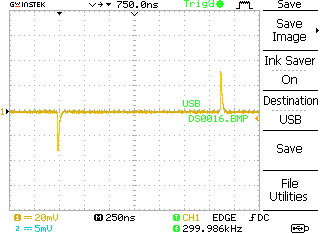
\includegraphics[width=0.5\textwidth]{MesswerteVersuch1/DS0016.png}	

					\caption{Leitungsabschluss mit Wellenwiderstand}
					\label{fig:DS0016}
				\end{figure}
				%TODO: Auswertung 3(d)

                Für den Fall, dass der Kabel mit seinem Wellenwiderstand abgeschlossen ist, würde man nur einen
                einzigem Peak erwarte, denn am Ende des Kabels wird das Signal nicht mehr reflektiert. Dies lässt sich
                gut in der Abbildung \ref*{fig:DS0016} erkennen.
\clearpage
% === Aufgabe 4 ===		

\subsection{Versuchsaufgabe 4: Klippkabel, Dämpfung}
			\begin{figure}[H]
				\centering
				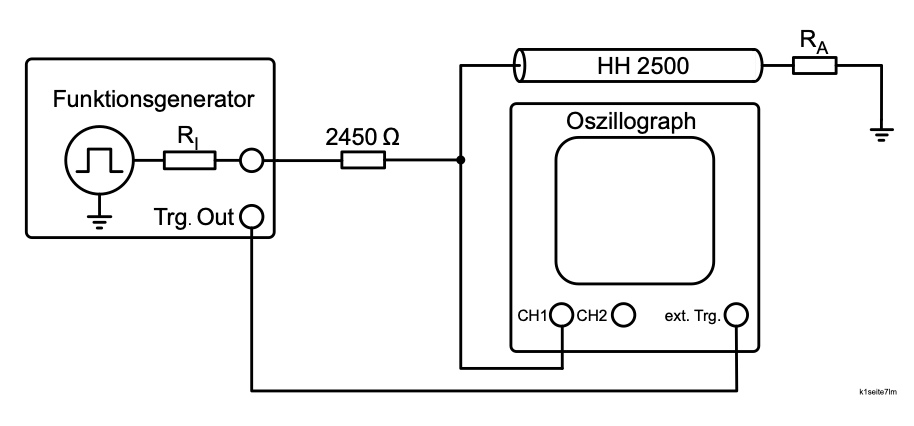
\includegraphics[width=0.5\textwidth]{figs/Aufbau_1_4_Klippkabel.png}
				\caption{Schaltplan für ein Klippkabel~\cite{anleitung}}
				\label{fig:aufbau_1_4_klippkabel}
			\end{figure}
			Zuletzt wird das Verzögerungskabel mit einem kürzeren, sogenannten Klippkabel, mit $\SI{0.7}{\meter}$ Länge ersetzt. Anstatt des Differenzierglieds wird ein Widerstand von $\SI{2450}{\ohm}$ eingebaut, der Widerstand vor dem Kabel wird entfernt. Der Funktionsgenerator wird auf eine Frequenz zwischen $\SI{10}{\kilo\hertz}$ und $\SI{80}{\kilo\hertz}$ eingestellt. Die Schaltverbindungen erfolgen mit $\SI{50}{\ohm}$ Koaxialkabeln. Dann wird unter den folgenden Umständen am Oszillographen gemessen:
			\begin{enumerate}[label=\alph*]
				\item Klippkabel mit $\SI{50}{\ohm}$ Abschluss, d.\ h.\ offen
				\item Klippkabel kurzgeschlossen
				\item Klippkabel kurzgeschlossen mit variierter Frequenz
				\item $\SI{2}{\meter}$ Klippkabel kurzgeschlossen 
			\end{enumerate}
Das Bild, das man bei einem offenen Vergrößerungskabelende bekommt, ist das folgende: 
				\begin{figure}[H]
					\centering
					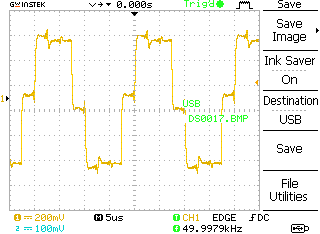
\includegraphics[width=0.5\textwidth]{MesswerteVersuch1/DS0017.png}
					\caption{Klippkabel mit offenem Ende}
					\label{fig:DS0017}
				\end{figure}
Hier sind die Peaks verschwunden und sind nun Stufen zu erkennen, die sich wegen des 
destruktiven Interferenz der beiden Signale erklären lassen, weil das Signal am offenen Ende
wieder reflektiert wird. 
\clearpage
Nun schließt man das Vergrößerungskabel an und erhält die folgende Abbildung:
				\begin{figure}[H]
					\centering
					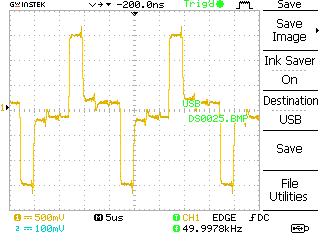
\includegraphics[width=0.5\textwidth]{MesswerteVersuch1/DS0025.png}
					\caption{Klippkabel mit kurzgeschlossenem Ende}
					\label{fig:DS0025}
				\end{figure}
                
 Hier sind die Plateaus wegen des Effekts der destruktiven Interferenz noch stärker beeinflusst, denn durch 
 den Kurzschluss wird die rücklaufende Welle gespiegelt. Das zeigt sich, indem die oberen Plateaus kürzer sind und die 
 mittlere Plateaus sich vergrößert. \\
 Variiert man die Frequenz ein wenig, erhält man die folgenden Bilder: 

				\begin{figure}[H]
					\centering
					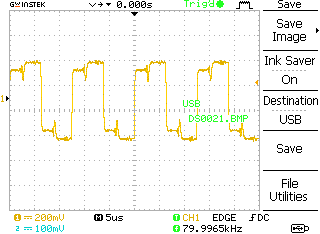
\includegraphics[width=0.5\textwidth]{MesswerteVersuch1/DS0021.png}
					\caption{Klippkabel mit offenem Ende bei $\SI{80}{\kilo\hertz}$}
					\label{fig:DS0021}
				\end{figure}
				\begin{figure}[H]
					\centering
					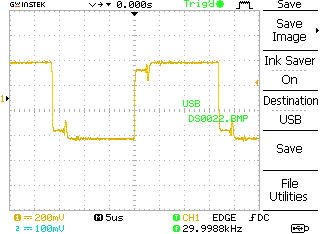
\includegraphics[width=0.5\textwidth]{MesswerteVersuch1/DS0022.png}
					\caption{Klippkabel mit offenem Ende bei $\SI{30}{\kilo\hertz}$}
					\label{fig:DS0021}
				\end{figure}
Wobei sich erkennen lässt, dass bei großeren Frequenzen Bereich,
 wo destruktive Interferenz auftaucht, vergrößert. Es ist wichtig anzdeuten, dass
 der Dauer des Impulses unverändert bleibt, weil das von dem Verzögerungskabel abhängt. \\
 Nun fügt man 2 weitere Klippkabel in dem Schaltsystem. Die Länge der geklippten Impulse wird durch 
 Ausnutzung von der Linearität zwischen Verzögerungszeit und Kabellänge. Da 2 weitere Kabel 
 angewendet werden, erwartet man eine dreifach-größerer Länge von Impuls.
\\
Bei den gekippten Impulsen kommt es zu einer Dämpfung. Hierdurch ist die Amplitude der rückreflektierten 
Welle geringer, weshalb bei der destruktiven Interferenz der Impuls nicht vollständig auf $0V$ eliminiert wird.
Die Dämpfung \( \beta \) berechnet sich aus der Eingangs- und Ausgangsspannung. Es gilt:

\[
\beta = \frac{20 \cdot \log_{10} \left( \frac{U_\text{out}}{U_\text{in}} \right)}{2 \cdot l}
= \frac{20 \cdot \log_{10} \left( \frac{U + U_2 - U_1}{U + U_1 - U_2} \right)}{2 \cdot l}
\]
Aus Abbildung \ref*{fig:DS0030} liest man ab, dass die Spannung $U=3V$, $U_1=0.21$ und $U_2=-0.36$ sind. 
\\ Es gilt also:  

\[
\beta = \frac{20 \cdot \log_{10} \left( \frac{U + U_2 - U_1}{U + U_1 - U_2} \right)}{2 \cdot l}
= \frac{20 \cdot \log_{10} \left( \frac{2{,}35}{3{,}65} \right)}{2 \cdot 21\,\text{m}}
= \frac{-3{,}834}{42} \approx -0{,}091\,\text{1/m}
\]


Die zugehörige Unsicherheit \( \Delta\beta \) ergibt sich nach der Gaußschen Fehlerfortpflanzung:

\[
\Delta \beta = \sqrt{
\left( \frac{\partial \beta}{\partial U} \cdot \Delta U \right)^2 +
\left( \frac{\partial \beta}{\partial U_1} \cdot \Delta U_1 \right)^2 +
\left( \frac{\partial \beta}{\partial U_2} \cdot \Delta U_2 \right)^2 +
\left( \frac{\partial \beta}{\partial l} \cdot \Delta l \right)^2
}
\]
Wobei $\Delta U_i =0.1V$ und $\Delta l =0.1m$ sind.
Was zusammen ergibt: 
\[
\beta = (-0{,}091 \pm 0{,}020)\,\text{1/m}
\]



 \begin{figure}[H]
    \centering
    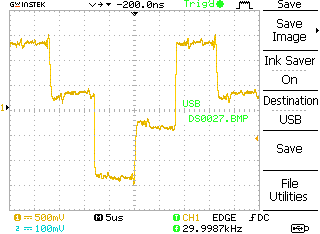
\includegraphics[width=0.5\textwidth]{MesswerteVersuch1/DS0027.png}
    \caption{Klippkabel aus 3 Teilstücken mit offenem Ende bei $\SI{30}{\kilo\hertz}$}
    \label{fig:DS0029}
\end{figure}
\begin{figure}[H]
    \centering
    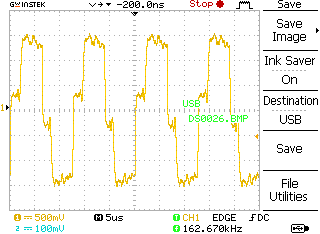
\includegraphics[width=0.5\textwidth]{MesswerteVersuch1/DS0026.png}
    \caption{Klippkabel aus 3 Teilstücken mit offenem Ende bei $\SI{160}{\kilo\hertz}$}
    \label{fig:DS0030}
\end{figure}

Dieser Wert ist unerwartet. Denn für den Kabel HH 2500 wäre die Dämpfung etwa $0.5 1/m$ in diesem Frequenzbereich.
Also besitzt der experimentell bestimmte Wert eine totale Abweichung von $82.2\%$. 
Dieses ist eine große Abweichung, welches dadurch erklärt werden kann, dass die Messung in zu niedrigem Spannungsbereich aufgenommen wurde.  
		
		%TODO Aufbau/Schaltskizze (beschrieben in wenigen Worten)
		%TODO Versuchsdurchführung: Messgrößen, unabh. Parameter, Messmethode, Einheiten, Genauigkeit, wie oft
		%TODO Abgezeichnetes Messprotokoll vorhanden?

		%TODO Auswertung (in Worten & Formeln)
		%TODO Formeln symbolisch und numerisch
		%TODO Runden
		%TODO Grafiken & Diagramme: Überschrift, Messwerte mit Fehlerbalken, (nur) gefittete Kurven, Achsenbeschriftung
		%TODO Fehlerrechnung und -diskussion
		%TODO Jede Tabelle eine Formel
	\section{Fazit}

    In diesem Versuch wurde untersucht, wie verschiedene Faktoren einer Leitung die Signalausbreitung beeinflussen. 
    Zunächst wurde mit einem Differenzierglied(ein Hochpass) ein Rechtecksignal abgeleitet, sodass nur noch seine 
    Peaks zu sehen waren. Hieran konnte man feststellen, dass der eingebaute Widerstand eine abschwächende Wirkung auf 
    das die Amplitude des Signals hatte und dass die Spannung flacher abgenommen hatte. Hiernach wurde das Verhalten 
    der Impulse an verschiedenen Kabelabschlüssen betrachtet.  Man konnte bestätigen, dass es zur Verzögerungszeiten 
    kommt. Außerdem konnten die Überlagerungen der reflektierten Wellen untersucht werden. Hierzu wurde die 
    Verzögerungszeit eine RG58C/U-Verzögerungskabels zu $ 5{,}83\pm 0{,}84\,\frac{\text{ns}}{\text{m}}$ bestimmt. Dieses stimmt mit dem Literaturwert 
    von $5 \frac{ns}{m}$ überein und ist daher glaubwürdig. Und zuletzt wurde ein Kippkabel benutzt, um verschiedene
     Abschlüsse zu untersuchen, wo Reflektionen, Dämpfungen und Überlagerungen untersucht werden konnten. 
     Und die Dämpfung des Klippkabels wurde zu $\beta = (-0{,}091 \pm 0{,}020)\,\text{1/m}$ berechnet, welches eine hohe Abweichung
      zum Literaturwerte $0.5 1/m$ hat. 
		%TODO Vollständiger Satz fürs Endergebnis
		%TODO Messergebnisse bewerten und evtl. mit Literaturwerten vergleichen
		%TODO Untersuchung Fehlerquellen (statistisch, systematisch, blödsinnig)
        \begin{thebibliography}{9}
        
        \bibitem{anleitung}
        \textit{Elektronikpraktikum -- Versuchsbeschreibungen}, Universität Bonn, 04.04.2025
        
        
        \end{thebibliography}



\end{document} 